% datum?
\documentclass[thesis=B,czech,hidelinks]{FITthesis}[2019/03/06]

\usepackage[utf8]{inputenc} % LaTeX source encoded as UTF-8

% my packages and stuff
\usepackage{todonotes}
\usepackage{xevlna}
% from https://tex.stackexchange.com/a/251025
\usepackage{relsize}
\usepackage{xspace}
\newcommand{\Rplus}{\protect\hspace{-.1em}\protect\raisebox{.35ex}{\smaller{\smaller\textbf{+}}}}
\newcommand{\Cpp}{\mbox{C\Rplus\Rplus}\xspace}
\usepackage[backend=biber,style=iso-numeric,sortlocale=cs_CZ,autolang=other,bibencoding=UTF8]{biblatex}
\addbibresource{mybibliographyfile.bib}

\hyphenation{NETCONF NETCONFu knihovnu knihovny}


\department{Katedra softwarového inženýrství}
\title{Nástroj pro konfiguraci a monitorování}
\authorGN{Václav}
\authorFN{Kubernát}
\authorWithDegrees{Václav Kubernát}
\author{Václav Kubernát}
\supervisor{Ing. Tomáš Čejka, Ph.D.}
% TODO: dopsat
\acknowledgements{Doplňte, máte-li komu a za co děkovat. V~opačném případě úplně odstraňte tento příkaz.}
% TODO: dopsat
\abstractCS{Bakalářská práce se zabývá vytvořením interaktivní konzolové aplikace sloužící ke konfiguraci síťových zařízení pomocí protokolu \textit{NETCONF}. Tento program slouží jako alternativa k dostupným, méně intuitivním, řešením. Toho dosahuje přívětivým uživatelským rozhraním implementovaným pomocí kniho\-vny \textit{replxx}.

Řešení využívá generátorů parserů, které jsou definovány deklarativně, knihovnu \textit{libyang} pro manipulaci s modelovacím jazykem \textit{YANG} a \textit{libnetconf} pro komunikaci přes protokol \textit{NETCONF}.
}
% TODO: dopsat
\abstractEN{This thesis focuses on creating an interactive console application with the purpose of configuring network devices over the \textit{NETCONF} protocol. This program serves as an alternative to available, less intuitive solutions. This is achieved mainly by creating a user-friendly interface implemented by the \textit{replxx} library.

The solution uses \textit{Boost Spirit X3} to create parsers defined declaratively, \textit{libyang} library for manipulating the \textit{YANG} modeling language, and \textit{\mbox{libnetconf}} for communication over \textit{NETCONF}.
}
\placeForDeclarationOfAuthenticity{V~Praze}
% TODO: zkontrolovat
\declarationOfAuthenticityOption{4} %volba Prohlášení (číslo 1-6)
% TODO: dopsat
\keywordsCS{netconf, yang, síťová konfigurace, konfigurace, cli, interaktivní cli, parsování}
\keywordsEN{netconf,yang,network configuration,configuration,cli,interactive cli,parsing}

\begin{document}

\begin{introduction}
Ke konfiguraci síťových zařízení existuje mnoho nástrojů. Pro klasického uživatele je nejlepší volba nějakého grafického rozhraní, ve kterém lze nastavit esenciální funkce jako například název nebo zabezpečení bezdrátové sítě. Pro síťové administrátory, kteří musí spravovat mnoho síťových zařízení najednou je ovšem takové řešení nevhodné, protože jej nelze používat v různých administrátorských skriptech apod. Je tedy nutné použít nějakou konzolovou aplikaci. V této práci se snažím implementovat program, který umožní administrátorům jednoduše a intuitivně konfigurovat síťová zařízení.

Pokud chceme konfigurovat zařízení po síti, je třeba nejprve způsob komunikace se zařízeními standardizovat. \textit{NETCONF} byl vytvořen organizací IETF jako standard pro konfiguraci síťových zařízení. \textit{NETCONF} neřeší způsob reprezentace konfiguračních dat, a proto byl pro tyto potřeby vytvořen modelovací jazyk \textit{YANG}. Více o těchto standardech píši v teoretické části práce.

V návrhové části práce se věnuji tomu, jakým způsobem lze program používat a rozebírám syntaxi programu.

Přestože je \textit{NETCONF} a \textit{YANG} v této práci klíčový, hlavním důvodem výběru této bakalářské práce je především použití generátoru parserů \textit{Boost Spirit X3}. Aplikace využívá tuto knihovnu k realizaci syntaxe, pomocí které je program ovládán. O \textit{Spiritu} se píše více v implementační části práce.
\end{introduction}
\chapter{Cíl práce} % TODO: mergenout s úvodem
Cílem práce je vytvořit konzolovou aplikaci, pomocí které lze vzdáleně konfigurovat zařízení pomocí protokolu \textit{NETCONF}. Aplikace bude intuitivní, uživatel by ji měl být schopný ovládat i bez detailní znalosti \textit{NETCONFu} nebo konkrétních modelů \textit{YANG}. K ovládání bude sloužit interaktivní mód, kde se uživatel zadává příkazy. Příkazy a jejich argumenty bude možné stiskem klávesy automaticky doplňovat.

\chapter{Teoretická část}
\section{YANG}
\textit{YANG}\cite{rfcYang} je jazyk sloužící k modelování konfigurace. Pomocí různých zabudovaných konstruktů lze vybudovat konfigurační strom, který logicky sdružuje různé druhy konfigurace, definuje kde lze jakou hodnotu nastavit, jaké mají datové typy apod. Kromě konfigurace podporuje \textit{YANG} i definování různých procedur. Kódování dat funguje pomocí XML\@.

Následovně definuji některé \textit{YANG} konstrukty, o kterých se zmiňuji v této práci:
\begin{description}
    \item[leaf]{neboli \uv{list} je nejnižší úrovní stromu a lze mu nastavovat hodnoty}
    \item[list]{neboli \uv{seznam} je způsob jak uložit více hodnot stejných parametrů}
\end{description}

\section{NETCONF}
\textit{NETCONF}\cite{rfcNetconf} je protokol vytvořený organizací IETF, sloužící ke vzdálené úpravě konfigurace síťových zařízení. Kromě konfigurace lze pomocí \textit{NETCONFu} implementovat zjišťování různých o stavu zařízení nebo se přihlašovat k různým oznámením. Je založen na na architektuře server-klient (můj program implementuje klientskou část). Při komunikaci přes \textit{NETCONF} zasílá klient serveru zprávy prostřednictvím XML-RPC\footnote{protokol založený na značkovacím jazyku XML, umožňující jednoduché volání vzdálených procedur}. Samotné zasílání zpráv na nižší úrovni probíhá přes protokol TLS nebo SSH\@.

Při zahájení komunikace si server i klient vymění \uv{hello} zprávu, ve které deklarují podporované \textit{capabilities}, což jsou definice operací, které dané zařízení podporuje. Základní \textit{NETCONF} podporuje několik typů zpráv. Ty, s kterými pracuje můj program jsou popsány níže.

\subsection{\texttt{<get>}}
Tato zpráva slouží k získání libovolné části podstromu. To může být konfigurace anebo stavová informace. Server odpovídá zprávou \texttt{<rpc-reply>} s požadovanými daty nebo zprávou \texttt{<rpc-error>} při chybě.

\subsection{\texttt{<get-config>}}
Tato zpráva se podobá zprávě \texttt{<get>}. Rozdíl je v tom, že pomocí \texttt{<get-config>} lze získat konfiguraci z různých lokací. \textit{NETCONF} podporuje tři druhy konfigurace:
\begin{description}
    \item[running]{aktuální platná konfigurace}
    \item[startup]{startovní konfigurace, která se aplikuje při spuštění zařízení}
    \item[candidate]{pracovní konfigurace, která může být zkopírována do running konfigurace}
\end{description}

\subsection{\texttt{<edit-config>}}
\texttt{<edit-config>} slouží k úpravě konfiguračního stromu na serveru. Klient zašle úpravy ve formě podstromu a vybere jestli chce tuto část sloučit s aktuálním podstromem, smazat, přepsat apod.


\chapter{Existující relevantní práce}
V tento moment existuje několik programů implementující klientskou část \textit{NETCONFu}. Jeden z nich je \textit{Netopeer2-cli} napsaná v jazyce C. Pro komunikaci přes \textit{NETCONF} využívá knihovnu \textit{libnetconf}. Výhodou je, že podporuje takřka veškeré konstrukty \textit{NETCONFu} včetně připojení přes TLS a SSH\@. Dalším programem je \textit{netconf-console}. Ta je napsána v Pythonu s pomocí knihovny \textit{ncclient}. Nevýhoda obou těchto aplikací je, že přestože jsou obě schopny konfigurace zařízení, jejich rozhraní není přívětivé jelikož pohlíží na věc z hlediska \textit{NETCONFu} a ne z hlediska toho, co chce uživatel konfigurovat. To v praxi znamená, že uživatel musí znát podrobně různé operace jako například \texttt{<get-config>} apod.


\chapter{Návrh}
Program je koncipován jako interaktivní konzolová aplikace. Silnou stránkou konzolových aplikací je možnost použití ve skriptech\footnote{skripty jsou jednoduché programy, používané k definování nějakých scénářů, například \uv{nastav nějaké údaje na nějakém zařízení}}. Uživatel může aplikaci použít jednak interaktivně, napojením terminálu na vstup programu a manuálním zadáváním příkazů, ale také dávkově, uložením příkazů do souboru a vložením tohotu souboru na vstup programu.


\section{Syntaxe}
Základní syntaxe programu vypadá takto:
\begin{verbatim}
/> <nazev prikazu> <prepinace> <argumenty>
\end{verbatim}
K pohybování ve stromu a nastavování hodnot jsem navrhl tyto příkazy:

\begin{description}
\item[cd]{přesun kontextu na jiné místo ve stromu}
\item[ls]{výpis uzlů stromu}
\item[get]{získání konfigurace ze vzdáleného serveru}
\item[set]{nastavení hodnoty leafu}
\item[create]{vytvoření instance listu nebo presence containeru}
\item[delete]{smazání instance listu nebo presence containeru}
\item[commit]{potvrzení aktuálních změn konfigurace}
\item[discard]{zrušení aktuálních změn konfigurace}
\end{description}

Na obrázku~\ref{ukazka} lze vidět příklad použití příkazů programu pro nastavení hodnotu leafu na \texttt{5}.

\begin{figure}
\begin{verbatim}
/> ls
Possible nodes:
example-schema:leafInt
example-schema:leafString
example-schema:someContainer
/> cd example-schema:someContainer
/example-schema:someContainer> ls
Possible nodes:
some_leaf
/> set some_leaf 5
/> commit
\end{verbatim}
\caption{Ukázková práce s programem}\label{ukazka}
\end{figure}

Aby bylo možné zadávat příkazy intuitivně, nabízí aplikace uživateli různé prostředky pro ulehčení zadávání vstupu, například různé klávesové zkratky pro pohyb v zadávaném textu, automatické doplňování stiskem tabulátoru (nebo jiné klávesové zkratky) a ukládání historie zadaných příkazů.


K pohybování konfiguračním stromem jsem zvolil podobný princip jako při pohybu adresářovou strukturou v počítači. Uživatel prozkoumává strom známými příkazy jako například \textit{cd}, nebo \textit{ls}. K manipulaci s hodnotami slouží například příkazy \textit{get} a \textit{set}.


\chapter{Implementace}
% TODO: dopsat něco o použitém jazyku a proč zrovna C++

\section{Fungování programu a jeho součásti}
Na obrázku~\ref{proud-dat} lze vidět, jak proudí data v programu. V následující části popisuji součásti aplikace, kterými data proudí.
\begin{figure}
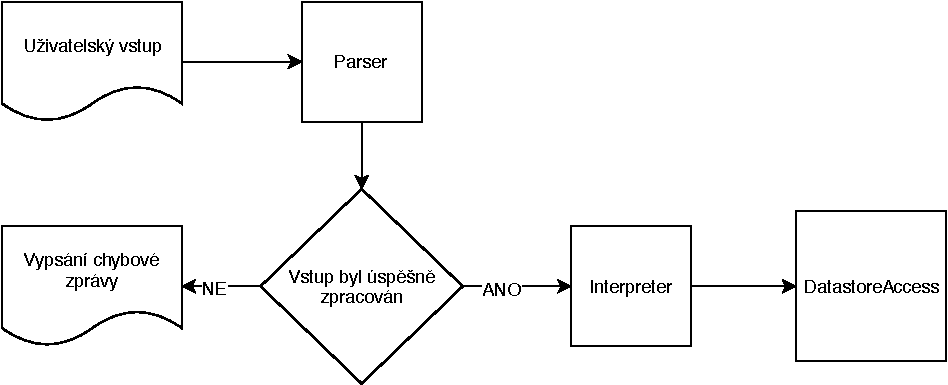
\includegraphics[width=.9\textwidth]{diagram}
\caption{Diagram proudu dat v programu}\label{proud-dat}
\end{figure}

\subsection{Uživatelské rozhraní}
Uživatelské rozhraní je poměrně přímočaré: program cyklicky načítá řádky uživatelského vstupu a zpracovává je. K interaktivnímu používání aplikace, je nutné implementovat nějaký způsob editace příkazové řádky. To zahrnuje především:
\begin{itemize}
    \item možnost úpravy aktuálního obsahu příkazové řádky před odesláním
    \item klávesové zkratkty \todo{Reword this}
    \item automatické doplňování příkazů pomocí klávesové zkratky
    \item ukládání historie příkazů
\end{itemize}
Ideální knihovna by měla mít nativní \Cpp{} rozhraní (ačkoliv lze v \Cpp{} relativně jednoduše použít i C knihovny) a být header-only, tedy, že k jejímu použití stačí přidat její hlavičkový soubor a všechny implementační detaily jsou obsaženy v něm.

Nejznámější knihovna využívaná k tomuto účelu je \textit{GNU Readline}\todo{ref?}. \textit{Readline} umožňuje editaci příkazové řádky pomocí mnoha klávesových zkratek, převzatých z textových editorů \textit{EMACS} a \textit{Vi} a také velmi intuitivní inkrementální automatické doplňování (tj.\ postupně doplňování vícenásobným stisknutím klávesové zkratky). Nicméně, vzhledem k tomu, že je již poměrně zastaralá, má pouze rozhraní v jazyce C, tudíž to není dobrá volba pro moji aplikaci. Další nevýhodou je její implementace: \textit{Readline} obsahuje přibližně 20 tisíc řádek kódu především kvůli kompatibilitě s mnoha emulátory terminálů. V dnešní době většina terminálových aplikací podporuje základní VT100 escape sekvence\todo{vysvětlivku} a tudíž není třeba zastaralé terminály podporovat.\todo{ref na linenoise readme.md}

Méně těžkotonážní variantou je knihovna \textit{linenoise}. Ta je oproti \textit{Readline} velmi malá -- má\todo{reword?} zhruba tisíc řádků. Její odnož \textit{cpp-linenoise} napsaná přímo v \Cpp{}, tudíž odpadají různé nevýhody použití jazyka C, a je header-only. Z hlediska funkčních požadavků \textit{cpp-linenoise} bohužel zaostává: nepodporuje mnoho klávesových zkratek (například kombinace klávesy Ctrl a směrových šipek) a automatické doplňování je pouze velmi jednoduché (neinkrementální).  Všechny tyto nedostatky řeší knihovna \textit{replxx}. Ta oproti \textit{linenoise} není header-only, nicméně velmi dobře napodobuje \textit{Readline} z hlediska podpory klávesových zkratek a automatického dokončování. Ve svém programu jsem tedy zvolil knihovnu \textit{replxx}.

% TODO: ukázat docopt.cpp (Ale někde jinde)

\subsection{Zpracování vstupu}
% TODO: intro o vstupu
% TODO: ukázat gramatiky

Ke zpracování gramatik příkazů je potřeba parser\footnote{česky syntaktická analýza; v mém programu část, která převádí textový vstup na strojově čitelný výstup}. Implementaci parseru lze provést manuálně, to ovšem může být u složitých gramatik velmi nepraktické, a proto je vhodné použít nějakou knihovnu, která dokáže parser vygenerovat. Na základě doporučení jsem použil knihovnu \textit{Boost Spirit X3}. Jednou z hlavních výhod knihovny \textit{Spirit} je, že gramatiky lze zádavat přímo do zdrojového kódu výhradně pomocí prostředků jazyka -- operátorů. To znamená, že není potřeba spouštět žádný preprocesor\footnote{program který transformuje zdrojový kód před jeho vlastním zpracováním}, který by převedl speciální syntaxi parseru do validního \Cpp{} kódu. Mimo to, výstup \textit{Spiritu} je přímo ve formě struktur \Cpp{}, takže není třeba výstupy parseru manuálně vytvářet. To ale s sebou nese jistou nevýhodu a tou je, že parser je taková černá skříňka, která špatně debuguje.
% TODO: Ukázka gramatiky napsané pomocí Spiritu
% TODO: dopsat gramatiky na základě datového modelu


% TODO: ukázat Boost Spirit
% TODO: ukázat libyang

\subsection{Interpreter}
Další součástí programu je interpreter. Vzhledem k tomu, že je \textit{Spirit} schopen získat příkazy od uživatele v podobně velmi dobře čitelné strojem, není složité podle nich implementovat správnou funkcionalitu. Práce interpreteru je v zásadě jen volání správných procedur třídy \texttt{DatastoreAccess}.

\subsection{DatastoreAccess}
\subsection{Přístup k úložišti konfigurace}
K vykonávání příkazů potřebuje interpreter přístup k datovému úložišti. Toto je implementováno pomocí abstraktního rozhraní \texttt{DatastoreAccess}. Tato součást obsahuje procedury k nastavování leafů na různé hodnoty a jiné metody na změnu konfigurace. V mé aplikaci budou implementována tato konkrétní rozhraní:
\begin{description}
    \item[NetconfAccess]{Třída implementující komunikaci pomocí \textit{NETCONF} s využitím knihovny \textit{libnetconf}}
\item[SysrepoAccess]{Třída implementující komunikaci se \textit{Sysrepo}\footnote{program, který používá \textit{Netopeer2} server pro ukládání dat} démonem}
\end{description}

\subsubsection{NetconfAccess}
% TODO: ukázat libnetconf2

\subsubsection{SysrepoAccess}
% TODO: ukázat sysrepo klientskou knihovnu

\subsection{Testování}
% TODO: ukázat doctest
% TODO: ukázat trompeloeil
% TODO: zmínit Catch

\subsection{Knihovna na logování?}
% TODO: spdlog, použito jen v netconf cpp wrapperu... od Honzy


\chapter{Vyhodnocení}
\section{Testování}
% TODO: testování přes doctest, především unit testy, ale i nějaký jiný (sysrepo.cpp)\@. hlášení bugů přes issue tracker, po opravení napsán test
\section{Porovnání s konkurencí}
% TODO: popsat, že ačkoliv moje aplikace nepodporuje 100 \% YANGu/NETCONFu, na základní použití stačí (hlavní cíl byl, upravovat konfiguraci bez znalosti YANG modelů a NETCONFu)
\section{Výsledky z nasazení}
% TODO: no, prej to Honza používá xD

\begin{conclusion}
% TODO: Něco dopsat sem, asi v závislosti na zbytku
\end{conclusion}

\printbibliography{}

\appendix

\chapter{Seznam použitých zkratek}
% \printglossaries
\begin{description}
    \item[GUI] Graphical user interface
    \item[XML] Extensible markup language
\end{description}

\chapter{Obsah přiloženého CD}

%\begin{figure}
%	\dirtree{
%            .1
%	}
%\end{figure}

\end{document}
